\documentclass{beamer}

\usepackage[czech]{babel}
\usepackage[utf8]{inputenc}
\usepackage{transparent}
\usepackage{pgfplots}
\usepackage{svg}
\usepackage{minted}

\newminted{yaml}{
	fontsize=\footnotesize, 
	frame=lines,
	bgcolor=bg,
	framesep=3mm
} 
\usemintedstyle{yaml}
               		

\setsvg{svgpath = img/}

\usepgfplotslibrary{dateplot}

\usetheme{metropolis}
\title{Minimalistický CI systém}
\date{}
\author{Autor: Martin Franc \\ Vedoucí práce: Ing. Jakub Jirůtka \\}
% \institute{FIT ČVUT}

\metroset{block=fill}

\begin{document}


\definecolor{bg}{rgb}{0.95,0.95,0.95}

\defverbatim[colored]\exampleCode{
\begin{yamlcode}
stages:
  - first
  - second
jobs:
  job1:
    env:
      test: "1"
    stage: first
    image: "alpine/3.5"
    commands:
      - apk update && apk add python python-tox
      - tox -e py36
    when: "PIPER_BRANCH == 'master'"
    after_failure:
      - cat build.log
\end{yamlcode}
}


\maketitle

% Cíle, motivace, rešerše, analýza, návrh, řešení, testování, souhrn udělané práce. Motivace a rešerše nemusí být, návrh a řešení lze nějak sjednotit. Víc obrázku s popisama, text v bodech. Co nejméně prázdných míst na slajdu.

\begin{frame}{Zadání}
\begin{block}{Cíle}
Navrhnout a implementovat minimalistický CI (Continuous Integration) systém vhodný pro
menší komunitní projekty a porovnat existující řešení.
\end{block}
\begin{itemize}
	\item Modulární podporu pro různá běhová prostředí,
	\item konfiguraci projektu pomocí textového souboru v repozitáři daného projektu,
	\item možnost paralelizace v rámci jedné úlohy,
	\item terminálové (přes SSH) a webové rozhraní,
	\item snadnou rozšiřitelnost a integraci na další systémy
\end{itemize}
\end{frame}

\begin{frame}{Analýza existujících řešení}
\begin{columns}[T,onlytextwidth]
\column{0.8\textwidth}
	Travis CI:
	\begin{itemize}
		\item \uv{Hostovaná} služba.
		\item Spjatý s GitHubem.
	\end{itemize}
	Gitlab CI:
	\begin{itemize}
		\item Správce projektů i CI systém.
		\item \uv{Self-hosted} i \uv{hosted}.
	\end{itemize}
	Buildbot:
	\begin{itemize}
		\item Framework.
	\end{itemize}
\column{0.2\textwidth}
 	\vbox to .6\paperheight{
 	\vfill
	\includesvg[width = 40pt]{travis-logo}
	\vfill
	\hbox{\hbox to 10pt{}\includesvg[width = 40pt]{gitlab-logo}}
	\vfill
	\includesvg[width = 40pt]{buildbot-logo}
	\vfill
	}
\end{columns}
\end{frame}

\begin{frame}{Návrh}
Návrh systému se řídil následující pravidly:
\begin{itemize}
	\item REST architektura,
	\item KISS a Unix filosofie,
	\item programovací jazyk Python 3.5+ a framework Flask,
	\item konfigurace integrace ve formátu YAML,
	\item LXD běhové prostředí.
\end{itemize}
\end{frame}

\begin{frame}{Architektura systému}
	\hfill
	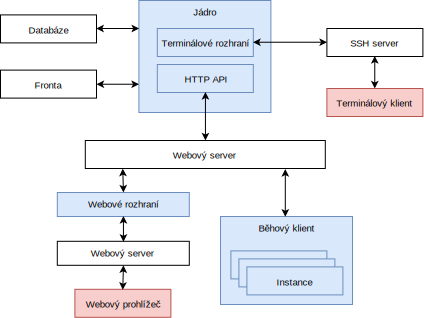
\includegraphics[height=.8\paperheight]{img/architektura_piper.pdf}
	\hfill
\end{frame}

\begin{frame}{Architektura jádra systému}
	\hfill
	\includegraphics[width=.88\paperwidth]{img/core.pdf}
	\hfill
\end{frame}

\begin{frame}{Entity}
	\hfill
	\includegraphics[height=.8\paperheight]{img/entity_piper.pdf}
	\hfill
\end{frame}

\begin{frame}{Testování}
\begin{itemize}
	\item Integrační a jednotkové testy s nástroji Tox a pytest.
	\item Mock u webového rozhraní.
	\item Použití kontinuální integrace při vývoji.
\end{itemize}
\begin{figure}
\includegraphics[width=150pt]{img/piper-ci-badges.png}
\caption{Ikonky na GitHubu}
\end{figure}
\end{frame}

\begin{frame}{Ukázka konfigurace integrace}
	\exampleCode{}
\end{frame}

\begin{frame}{Výsledek práce}
\begin{itemize}
	\item Rešerše existujících řešení.
	\item Modularita pomocí HTTP API.
	\item Minimálnost je dosažena KISS filosofií.
	\item Sledování stavu integrací a administrace systému v terminálovém rozhraní.
	\item Sledování stavu integrací ve webovém rozhraní.
	\item Různá běhová prostředí.
	\item Paralelizace v rámci fáze.
\end{itemize}
\end{frame}

\begin{frame}{Přínosy práce}
\begin{itemize}
	\item 1k LoC.
	\item Minimální počet závislostí.
	\item Nízké požadavky na systémové prostředky.
	\item LXD běhové prostředí.
	\item Instalace přes Pip.
	\item Autentizace pomocí asymetrických klíčů.
	\item CLI jako \uv{first-class citizen}.
\end{itemize}
\end{frame}

\begin{frame}[standout]
	Děkuji za pozornost.
\end{frame}

\end{document}